% Introdução
\chapter{Introduction}

Brazilian people are regarded throughout the world as being very warm and friendly, but at the same time, the high crime rate has given Brazil a reputation as a very dangerous place both for residents and tourists. Traditionally,, the crime rates in Brazil have been higher than those in other countries, even when compared to its neighboring countries which are in the similar position of being emerging nations (e.g., Argentina, Chile, Uruguay, Paraguay, and others) or underdeveloped (as in the case of Haiti)\cite{Harrendorf2010}

Recent available statistics show that in 2012, Brazil recorded 22.8 homicides per 100,000 inhabitants, which is much higher than what the World Health Organization considers to be acceptable (i.e., 10 homicides per 100,000 inhabitants). It is also worth mentioning that the homicide rate rose by 11\% in Brazil in the period 2010 - 2012.\cite{Murray2013}

Hence, crime is a major concern in Brazil, especially in the larger cities. Both the police and the press have stated that crime is becoming more widespread, especially in the evenings and late at night. Street crime is a particular problem\cite{OSAC2015} and violent crimes are regularly being committed (notably murder, kidnapping, carjacking, armed assault and burglary). Among the wide range of crimes being committed in Brazil, the field of transport -safety has attracted special attention because of the sharp rise of incidents involving vehicle thefts, and in particular, violent crimes on urban buses.

For instance,the authorities in Fortaleza/CE reported a total of 2,517 thefts on buses in 2013, an average of 6 incidents daily and showing an increase of 309\% when compared to 2012 (615)\footnote[1]{Jornal de Hoje - Cotidiano - http://www.opovo.com.br/app/opovo/cotidiano/2014/02/11/noticiasjornalcotidiano/3204855/fortaleza-registrou-media-de-seis-assaltos-a-onibus-por-dia-em-2013.shtml . Accessed in December 10th, 2015}. These occurrences are frightening to both drivers and conductors, who are exposed to these incidents every day since these traumatic experiences occur in their workplace.

Real life testimony and statistical data reveal the sharp rise of crime in the North-East of Brazil. This is illustrated in Figure\ref{fig:fortal} which shows data from the Public Transport Companies Union in the State of Ceará - SINDIONIBUS\footnote[2]{Public Transport Companies Union in the State of Ceará - SINDIONIBUS. http://www.sindionibus.com.br. \textit{Accessed on December 1st , 2012.}} which provides information about the number of assaults that occurred in Fortaleza in the public transport system in the years 2012 and 2013.

\begin{figure}[htb!]
	\centering
  	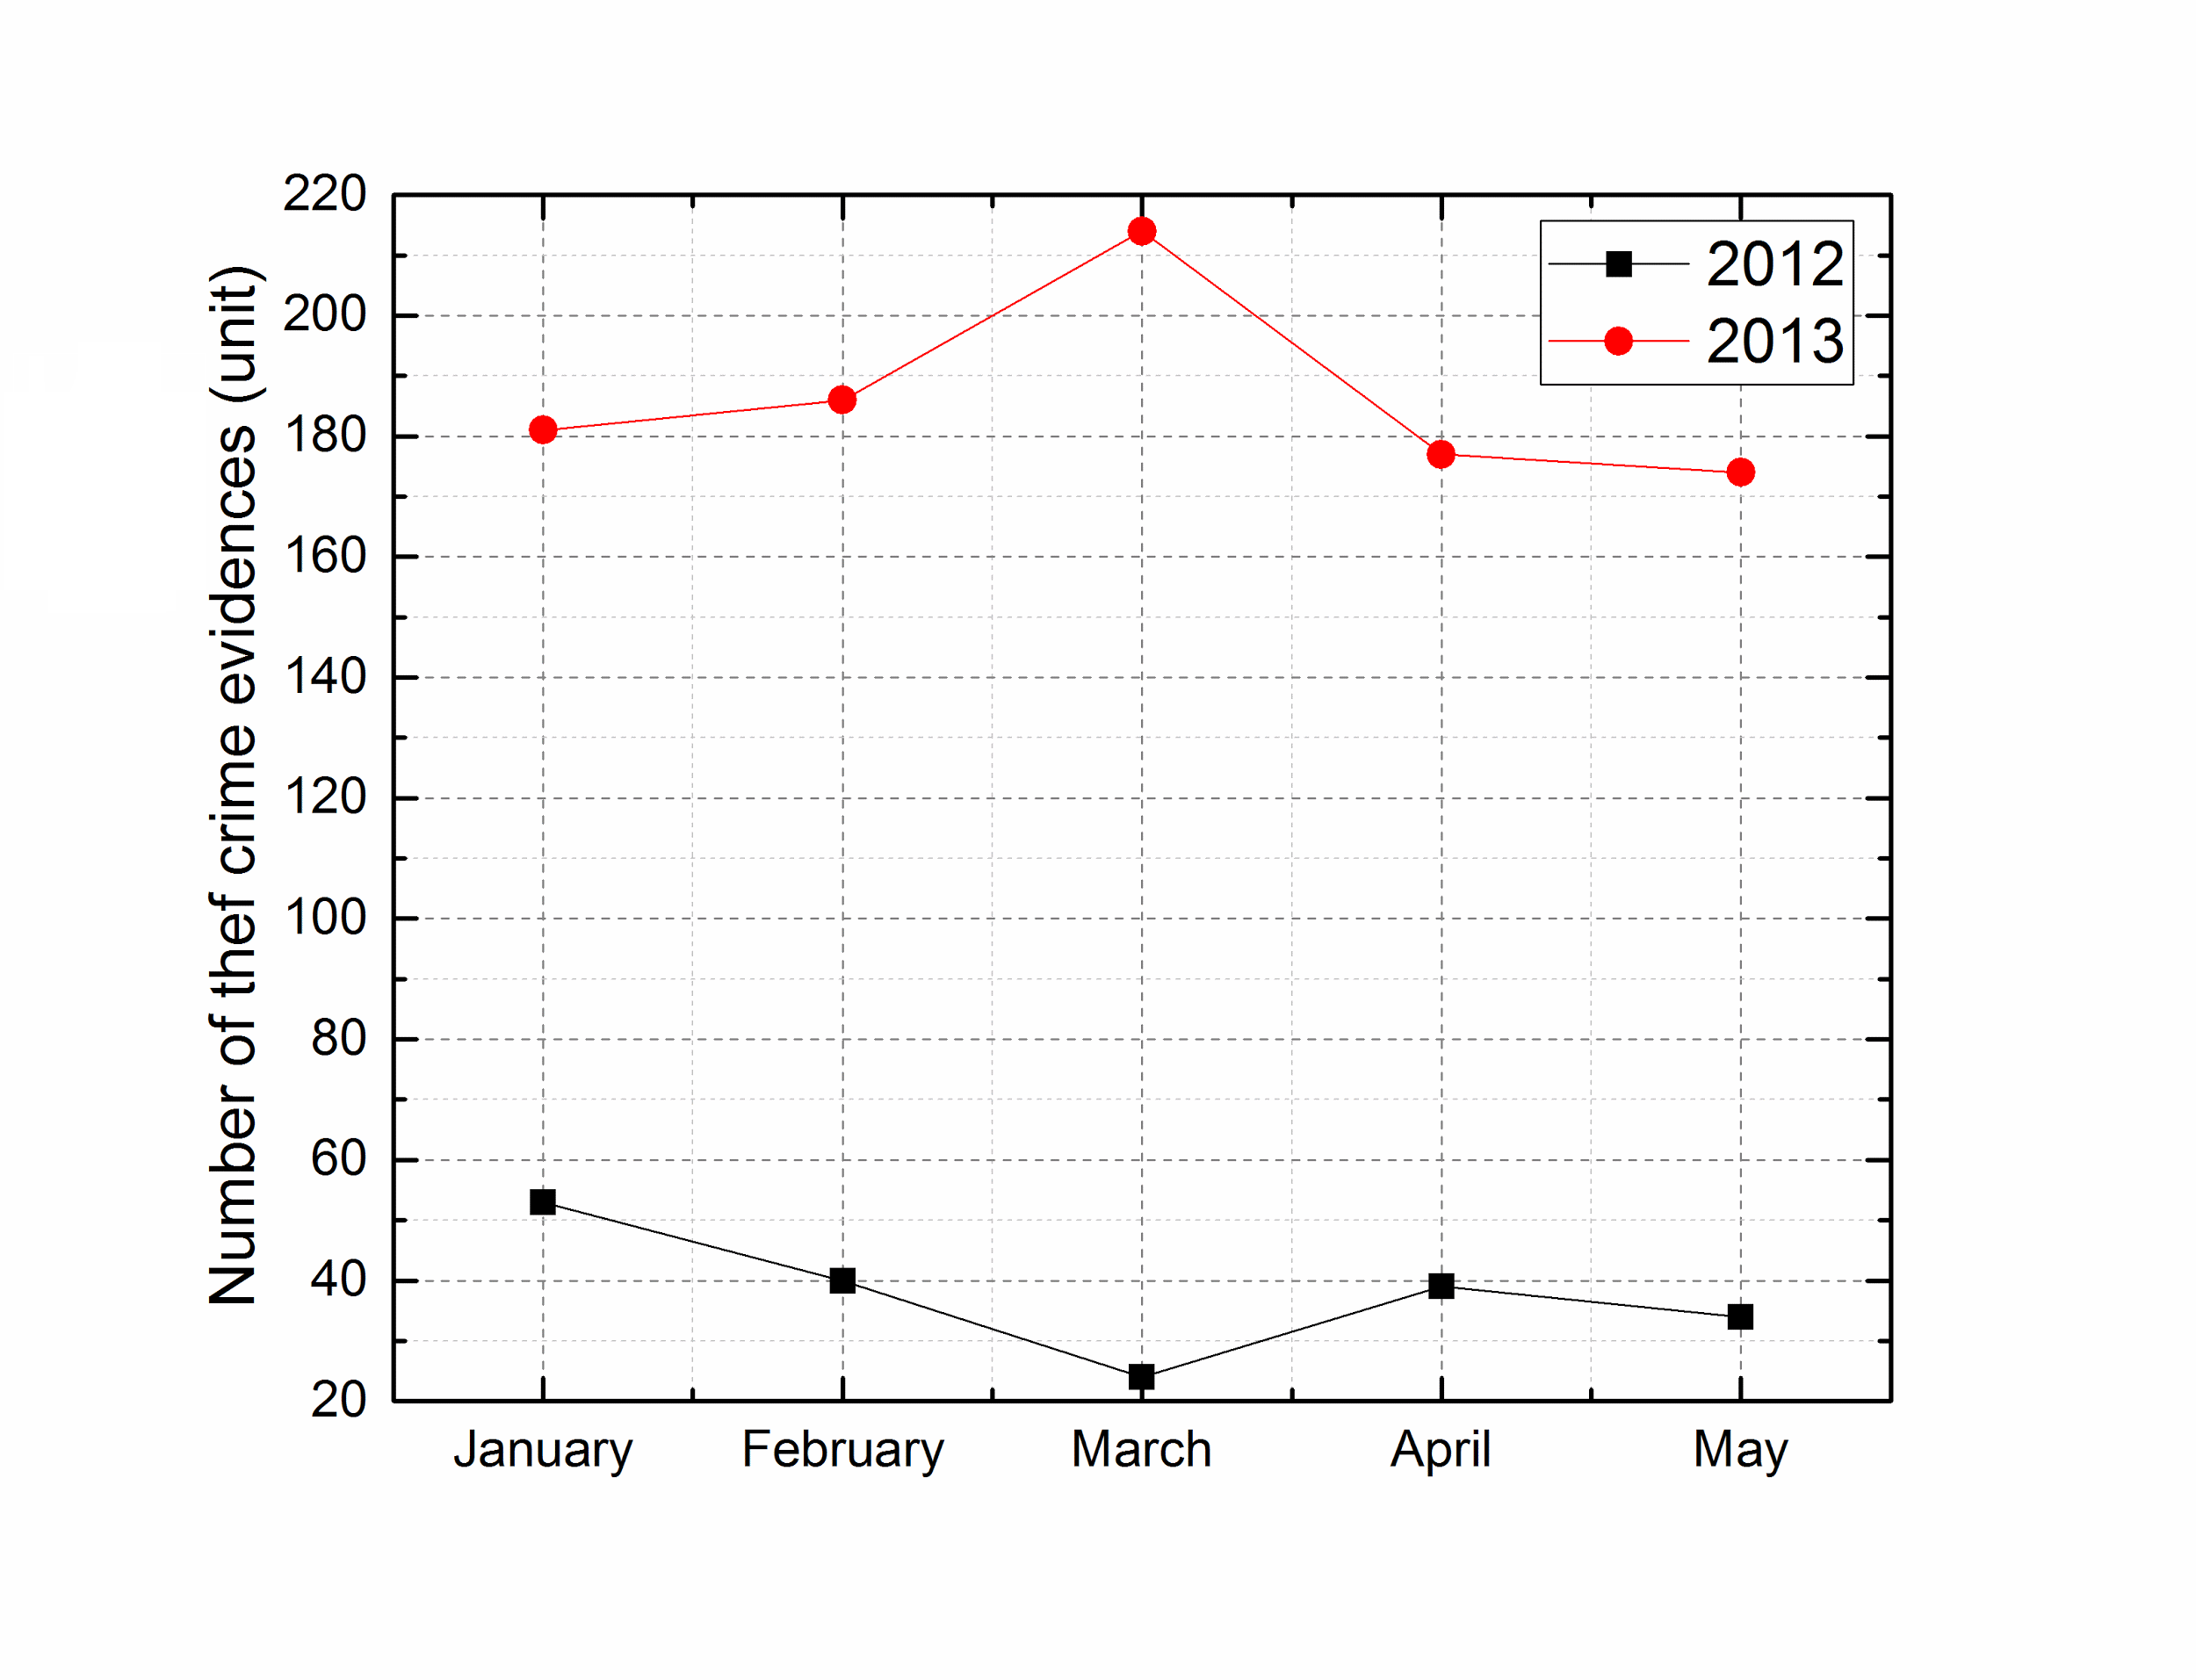
\includegraphics[scale=0.20]{Imagens/intro_fortaleza.png}
  	\caption{Numbers of witnessed crimes of theft in Fortaleza (2012 - 2013).}
  	\label{fig:fortal}
\end{figure}

In Natal, the Figure\ref{fig:natal} highlights the number of recorded events, based on information supplied by the Urban Public Transport Companies Union in the city of Natal - Seturn\footnote[3]{Urban Public Transport Companies Union in the city of Natal - SETURN. http://www.seturn.com.br. \textit{Accessed on December 1st , 2014.}}, which showed an increase of 198. 43\% in the rate of witnessed thefts from the year 2012 to 2013.

\begin{figure}[htb!]
	\centering
  	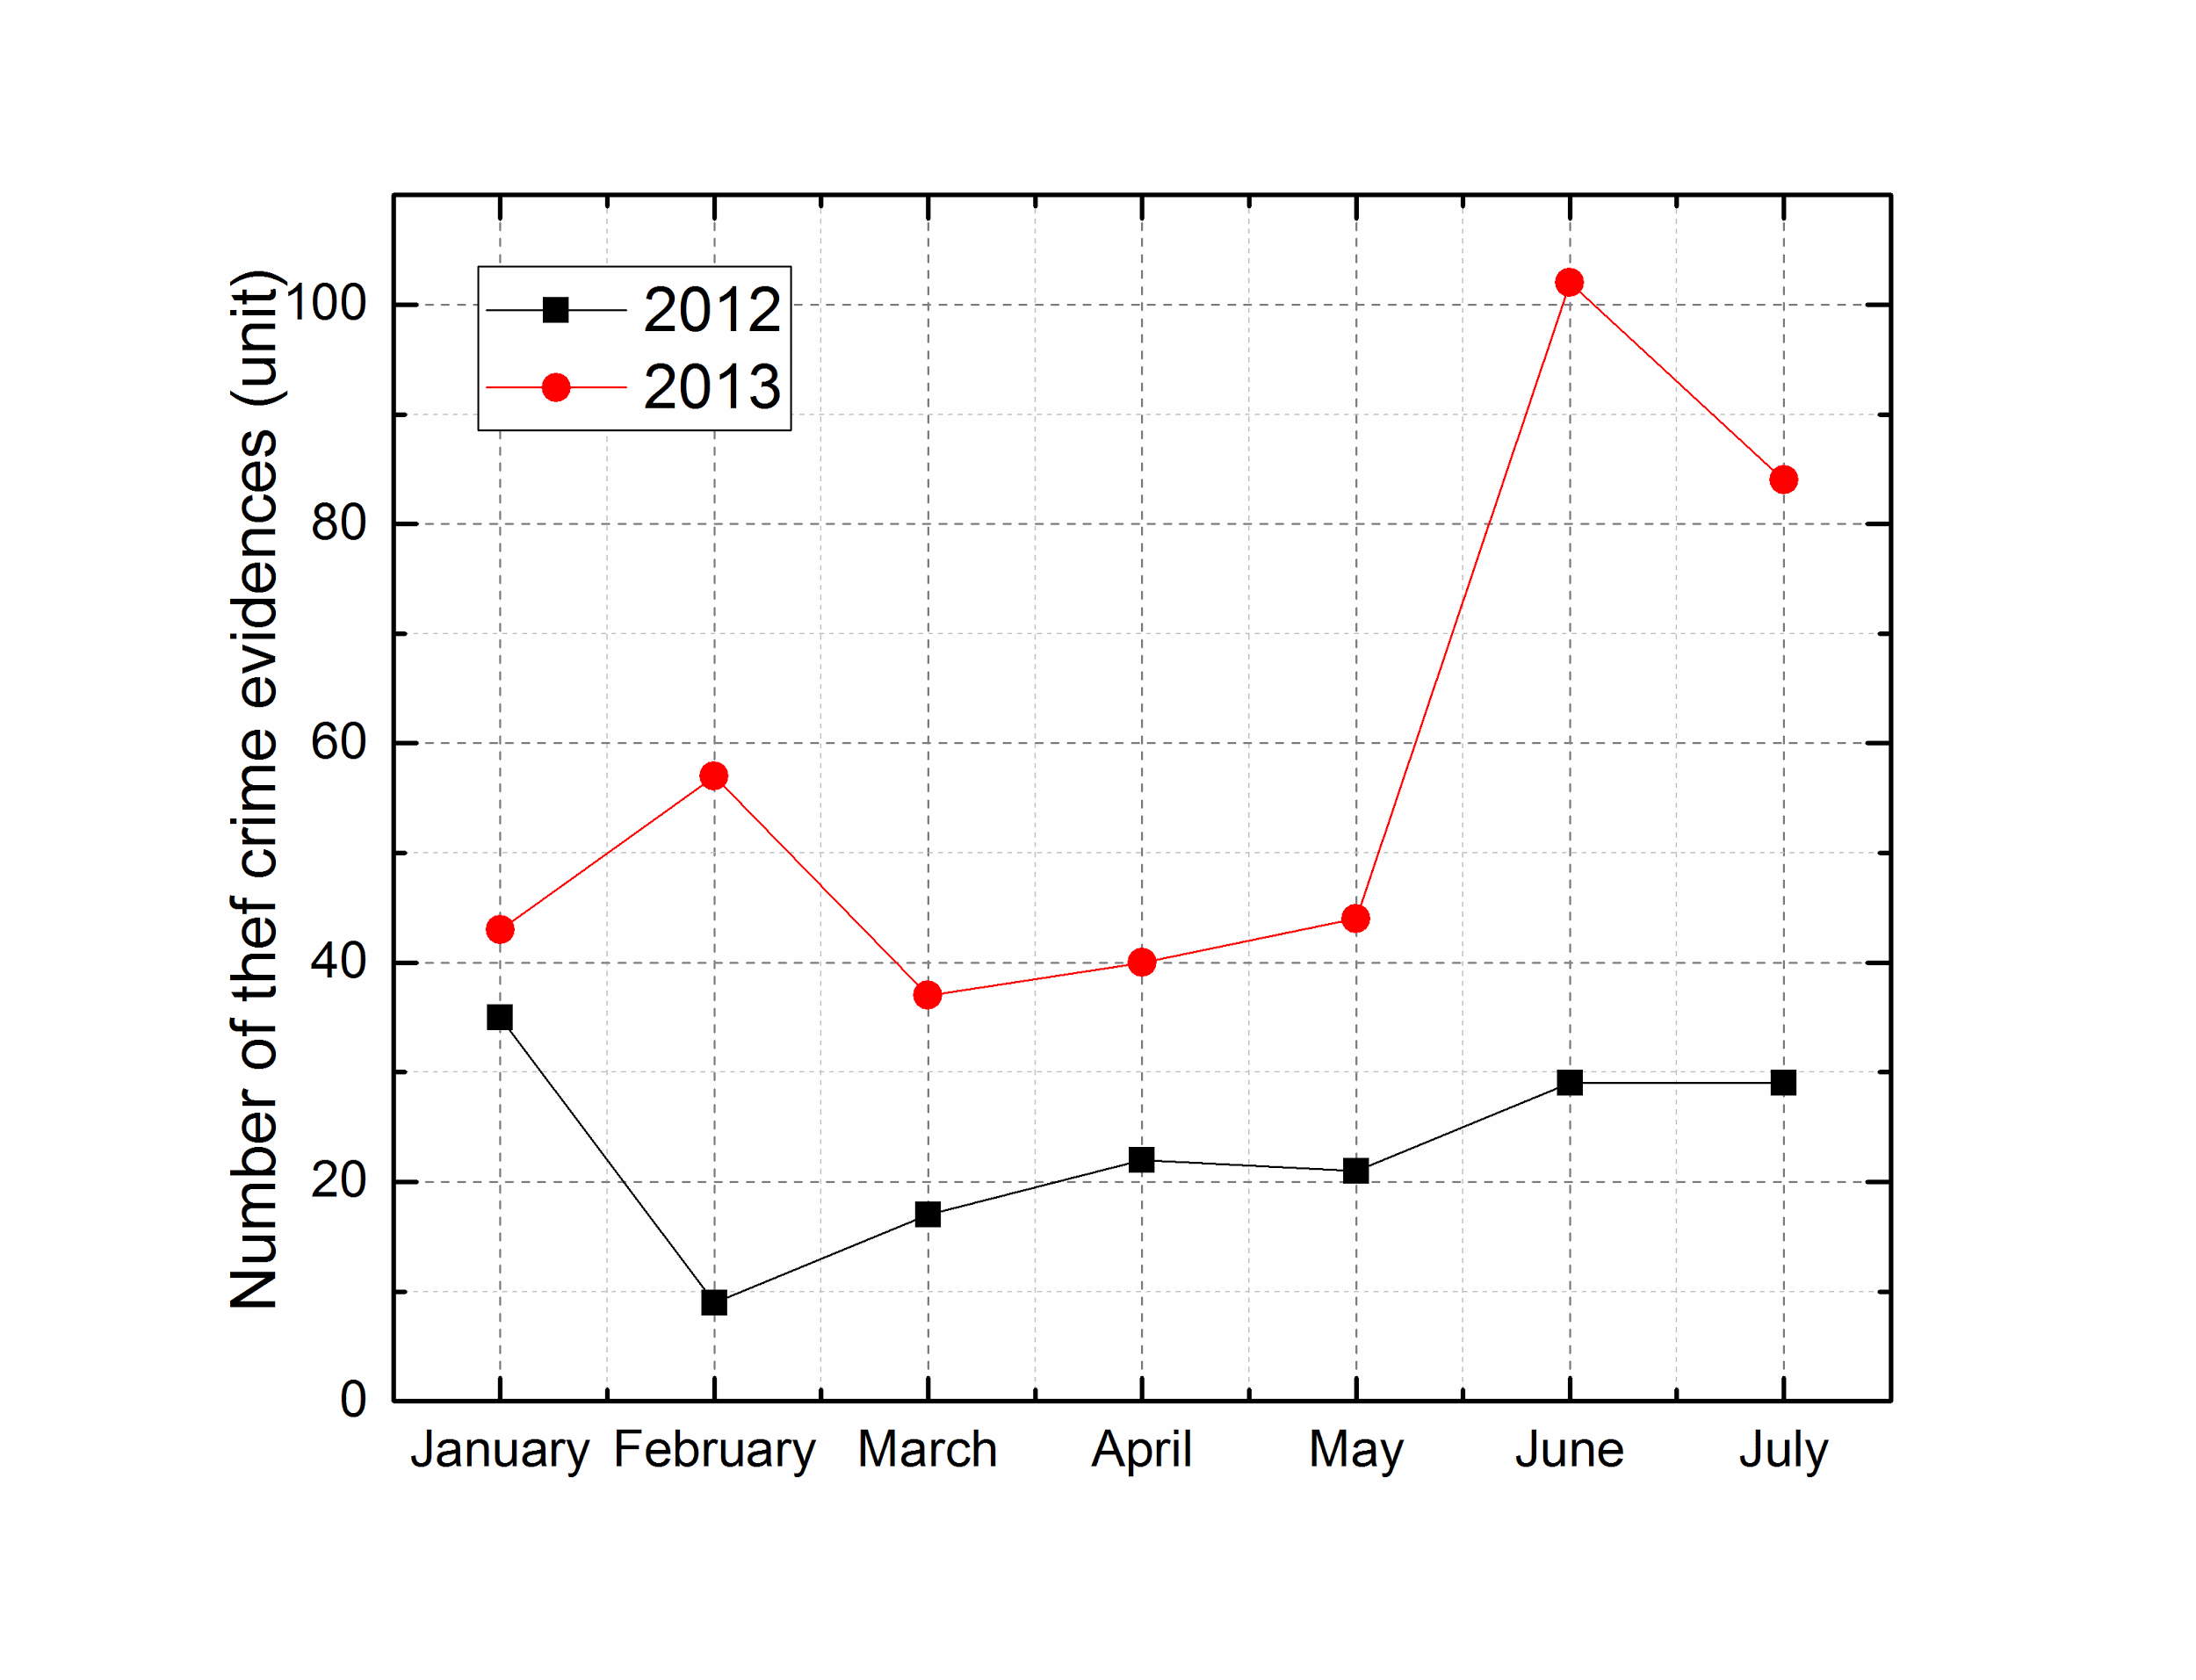
\includegraphics[scale=0.20]{Imagens/intro_natal.png}
  	\caption{Numbers of witnessed crimes of theft on buses in Natal (2012 - 2013).}
  	\label{fig:natal}
\end{figure}

The crimes on urban buses are mostly carried out with selected weapons (guns, sharp knives, etc.) which are primarily aimed at making the victim afraid, and if there is any resistance or sudden reaction on the part of the victim, the criminals often kill them in cold blood. This naturally increases the number of murders committed each year and makes Brazilian citizens feel extremely insecure. In light of this, transport safety in Brazil has become a real concern for the government and authorities, which are always seeking effective ways of eradicating (or at least alleviating) this social evil. The traditional model adopted by police authorities is 100\% reactive, since it relies on human intervention in the form of a request to assist the crime victim ( through the use of emergency call services, in-vehicle panic button systems, constant monitoring of surveillance cameras, and the like). 

However, the citizens (the users or drivers) are scared to make use of these available services because they might face retaliation from the criminals, and either be killed during the crime or later on in a revenge attack. As a result, over 90\% of the criminal offences are never detected by the police, and when criminals are arrested , only about 5\% to 8\% of the murderers are punished\footnote[4]{Nation Master - Brazil Crime Stats - http://www.nationmaster.com/country-info/profiles/Brazil/Crime. Accessed in December 10th, 2015.}; this leads to a feeling of impunity among the perpetrators.

Thus, it is essential to make use of to Information and Communication Technology (ICT) for event detection and subsequent response by means of automated systems. Smart Environments is a potential research field that leverages ICT to control urban violence \cite{Droege1997}. A Smart Environment can be characterized as a space with various network devices, which embeds processing power and sensing systems that cooperate with each other in assisting end-users to carry out their tasks more efficiently. 

A Smart Environment must be able to: (i) recognize the users and their circumstances; (ii) have a prior knowledge of the environment; (iii) produce new services in real-time in areas such as entertainment, security, health, housework, the work environment, information outlets, computing, communication, etc.; (iv) allow access to the services and features provided by a Smart Environment, and take account of the location and the time when the event occurs.

A successful applicability of Smart Environments is Smart Cities \cite{Komninos2006}, which refers to a physical environment and adopts an ultimate ICT embedded in the physical objects and environment in which we live. The field of Smart City is increasingly attracting the attention of the research community because it offers the prospect of deploying new and innovative ICT to boost urban services of a better quality, performance and interactivity since it is able to provision sustainable services, offer a better quality of life, and cater for both the public and the government.

Smart City services are multisector, and include the government, transport and traffic management, and the energy, health-care, water and sanitation sectors. Smart City applications are planned with the aim of improving the management of urban traffic and provides real- time responses to challenges.

Smart Surveillance\cite{barros2014} is a technology that adopts advanced processing techniques from the data gathered of surveillance subsystems (cameras and/or microphones) spread across a Smart City area. It seeks to process multimedia data obtained from a target monitoring zone, with the goal to detect/track security threats, such as a person's suspicious behavior or holding a dangerous object (knife or gun).

Smart Surveillance is mostly used in pedestrian zones (squares, sidewalks, shopping centers/banks, etc.), which have benefited from a high rate of crime incident detection, since the devices are installed in fixed places, and interconnected with standard communication techniques to the control center of the police authorities. Figure\ref{fig:fixed} provides an example of devices installed in fixed places and deployed through wide broadband in New York City - EUA.

\begin{figure}[h!]
	\centering
   	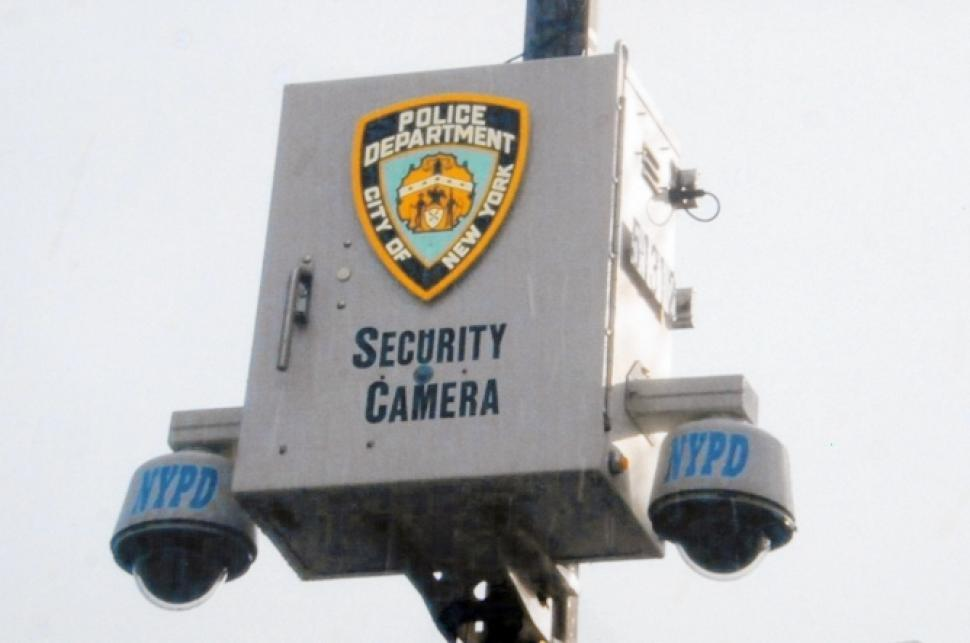
\includegraphics[scale=0.45]{Imagens/intro_fixed.png}
	\caption{Surveillance subsystem at a fixed place}
	\label{fig:fixed}
\end{figure}

Smart Transportation-Safety systems is an area in Smart Cities transportation\footnote[5]{Smart Transportation Alliance - http://smart-transportation.org/. \textit{Accessed in December 10th, 2015.}} that has attracted special attention in this study, because it involves innovative strategies for dealing with security threats in transport system. The main idea consists of exploiting an in-vehicle ICT that is integrated into other Smart City systems (control centers, intelligence authorities, cyber-physical systems, etc.) to reduce fatalities. 

In the scope of this dissertation, Smart Transportation-Safety is suited to the problem of crime incidents in Brazilian urban buses, since it provides ICT with the ability to cope with the violent incidents described above, and thus provide more safety for the public, as well as to drivers and conductors. With the support of specific multimedia sensors (e.g., video surveillance cameras and/or microphones) along with specific data analytics afforded by signal-processing techniques, it will be likely possible to automatically detect criminal threats at the time they are carried out, and hence trigger the most appropriate crime assist with more agility.

The dissatisfaction with the inefficient model currently adopted by police authorities in dealing with the crime incidents on buses, as well as the sharp rise in the re-incidence rates, forced urban bus companies constantly searching for alternative strategies that can assist in keeping criminals out of urban buses, or at least, hesitate before committing in-vehicle crimes. Initial measures have resulted in the installation of video cameras and GPS location sensors for the entire fleet, to allow the interior of the buses to be monitored (off-line), as well as to carry out tracking. 

With regard to video surveillance, the employers are in charge of analyzing the offline video files compiled by the cameras after an incident. This reactive scheme is naturally an inefficient way of avoiding an incident, especially fatalities, because it depends exclusively on humans operation to analyze the video for identifying events of potential security threats after physical occurrence, which may be doomed to failure in stressful conditions or other adverse factors. Rather than this, it would be helpful to enable the authorities to find out a criminal's identity and the way the crime has been committed.

Smart Transportation-Safety can be defined as a set of systems that feature computing capabilities to collecting, processing, and analyzing multimedia data for identifying events of potential security threats (e.g., robberies, fights, accidents, kidnappings, etc.) in the transportation service \cite{Anwar_Hossain}. Hence, Smart Transportation-Safety system is an asset for anticipated procedures, helping to mitigate the problem of crime on urban buses in an accurate and effective way, with more accuracy and agility in comparison to humans.

The evolution of multimedia signal processing techniques (audio, images and video), as well as pattern recognition, has led to the development of smart tools with great capacity for accurate detection and rapid decision-making \cite{Schonfeld2010}. Within the scope of this proposal, the target Smart Surveillance-based Transportation-Safety system is introduced as a system approach featuring a set of interworking and autonomous technologies. In another words, the targeted system must collect multimedia data through sensors in the bus cabin and processing them in real-time to automatically identifying events of potential security threats at bus cabins.

Other countries in Europe, Asia and North America have successfully adopted a similar technical form of Smart Surveillance-based Transportation-safety system and, achieved a reduction in crime\footnote[6]{Homeland Security News Wire - http://www.homelandsecuritynewswire.com/study-shows-surveillance-cameras-reduce-crime-some-cases. \textit{Accessed on December 10th, 2015.}}. Moreover, these  applications can be deployed to improve efficiency in prevention, affording a proactive approach. For instance, when an incident is detected, this application can embody capacities to alert the most appropriate authorities (e.g. a police vehicle with expertise on crime , which is located close to the area to deal with the incident by attempting to save the lives of the victims and punish the criminals.

To achieve this, the Smart Surveillance-based Transportation-Safety systems require the assistance of reliable communication technologies (broadband, mobile and quality guaranteed) and smart devices (sensors/actuators such as pan-tilt-zoom cameras). These are employed to support the following: a) mobility at high speed, b) a reliable transmission of data, c) the ability to keep the system available for ubiquitous access, and d) a means of switching/ moving directly to the Smart City zone to change the standard behavior. 

Thus the data produced will help both to assist in solving crimes and to prevent them by triggering reactive mechanisms which act as protective measures or, depending on the nature of the situation, can assist in saving victims.

On the basis of the the major concerns facing transportation-systems \cite{Karagiannis2011}, including scalability, ubiquitous access to sensory data, event processing overhead, and massive storage requirements, cloud Computing plays a key role in supporting several applications for high-performance and high-reliability perspectives \cite{Anwar_Hossain}. Cloud Computing is a successful concept that combines many fields of widely used computing paradigms to provide a service infrastructure that can reduce the costs of managing hardware and software resources \cite{Hayes2008}. 

In Smart Surveillance-based Transportation-Safety systems, cloud computing can benefit a powerful and scalable service infrastructure for large-scale storage, processing, and flexible dissemination of data/information. Cloud computing includes hardware, software systems, and the applications delivered as services over the Internet \cite{Xinhui2009}.

For the purposes of this work, we strongly believe that the combination of Cloud Computing with Smart Surveillance-based techniques is key enabler for an efficient Smart Transportation-Safety system, and will enhance public safety in Smart Cities by enabling the deployment of autonomous and real-time crime assist at bus service.

The resulting solution envisions to assist police authorities in finding the location of the crime, and thus getting the ability to respond to the incident efficiently (more agile and accurate). However, it is not a trivial task to deploy this system by facing the following challenges:

\begin{itemize}
\item Affording in-vehicle smart video surveillance subsystem with capacities to detect the occurrence of crime threats in real-time and with high-accuracy. To that, an efficient video processing algorithm, considering the high noise conditions on the bus cabin, plays a fundamental role on this process;

\item Deploying a cloud-enabled infrastructure, acting as a front-end between target vehicles surveilled and available crime assist units. The cloud infrastructure is envisioned to provision high-performance storage and processing (under smart computing design), as well as affording services with high-reliability, -accessibility and -availability;

\item Supporting event-driven mobile applications for use by crime assist unities. The event-driven mobile application is connected to the cloud service infrastructure to provide crime assist unities metadata (information about location, expertise, capabilities, etc.). Moreover, the cloud service infrastructure uses the event-driven mobile application to call crime assist, providing metadata about a detected security threat.

\end{itemize}

The challenges listed hereinabove are the basis for us to derive the motivation that is highlighted in the following section.

\section{Motivation}

To the best of our knowledge, there are no current works in the literature neither in the market that suit all the challenges described in the last section for affording efficient cloud-enabled Smart Surveillance-based Transportation-safety systems. This is the motivating factor that has driven this work and gives it global significance within both the research community and industry. Moreover, the resulting solution set out in this work is designed to help enhance aspects of public transportation-safety in Smart Cities. 

This is because, among other factors, it allows: (i) police authorities to respond to crime incidents with agility; (ii) city authorities to effectively plan city services and security; (iii) an improved quality of life for citizens and police authorities; (iv) plans for new applications to improve current strategies for public safety with proactive actions; (v) a greater degree of safety for the city.

\section{Objectives}

The main objective of this dissertation aims at evolving safety in transportation systems through exploiting emerging technologies in the research fields of ubiquitous and smart computing. The resulting approach includes designing a framework for loud Computing-assisted Smart Surveillance-based Transportation-Safety systems, and evaluating the architecture in a real testbed. In pursuing this goal, the specific aims that must be carried out to achieve the overall objective can be described as follows:

\begin{itemize}
\item Designing, implementing and evaluating a generic video processing mechanism for embedding the bus cabin system with smart surveillance camera subsystem. The smart surveillance camera is in charge for automatically detecting in-vehicle crime incidents, and sending the corresponding metadata to a cloud service infrastructure;
\item Designing, implementing and evaluating a cloud service infrastructure embodying applications that provision the following set of cloud services: (i) storage (for bookkeeping metadata of crime event detection produced by in-vehicle smart surveillance subsystems); (ii) multimedia processing (to classify the crime event detected by in-vehicle smart surveillance subsystems); and (iii) event notification (to select and call the best suited crime assist unit).
\item Designing, implementing and evaluating a mobile application that operates in a event-driven approach for lightweight behavior (allowing accessibility, survivability, best performance). The event-driven mobile application is the target for event crime notifications from the cloud service infrastructure, seeking to call crime assist;
\item Deploying the resulting framework on a real TestBed, for obtaining perspectives of accurate assessments and insights on the work proposal with use case;
\item Disseminating the obtained results in conference proceedings and journals that are certified and recognized by the Qualis\footnote[7]{CAPES/MEC. http://www-periodicos-capes-gov-br.ez18.periodicos.capes.gov.br/. \textit{Accessed on  January 30th, 2015.}} platform.
\end{itemize}

\abrv[3G -- Third Generation]{}
\abrv[CCTV -- Closed Circuit Television]{}
\abrv[CPU -- Central Processing Unit]{}
\abrv[DCD -- Dominant Color Descriptor]{}
\abrv[DOT -- Dominant Orientation Templates]{}
\abrv[EC2 -- Elastic Compute Cloud]{}
\abrv[EHD -- Edge Histogram Detector]{}
\abrv[FP7 -- EU Framework Program 7 for Research and Innovation]{}
\abrv[GPS -- Global Position System]{}
\abrv[Haas -- Hardware as a Service]{}
\abrv[IaaS -- Infrastructure as a Service]{}
\abrv[ICT -- Information and Communication Technology]{}
\abrv[IoT -- Internet of Things]{}
\abrv[IP -- Internet Protocol]{}
\abrv[IR - Infra Red]{}
\abrv[ISIS -- Intelligent Sensor Information System]{}
\abrv[JNI - Java Native Interface]{}
\abrv[NIST -- National Institute of Standards and Technology]{}
\abrv[PaaS -- Platform as a Service]{}
\abrv[PC -- Phase Correlation]{}
\abrv[PLS -- Product Lines Software]{}
\abrv[QoE -- Quality of Experience]{}
\abrv[QoR -- Quality of Recognition]{}
\abrv[QoS -- Quality of Service]{}
\abrv[RF -- Radio Frequency]{}
\abrv[S3 -- Simple Storage Service]{}
\abrv[SaaS -- Software as a Service]{}
\abrv[SIFT -- Scale-Invariant Feature Transform]{}
\abrv[SETURN -- Urban Public Transport Companies Union in the city of Natal]{} 
\abrv[SINDIONIBUS -- Urban Public Transport Companies in the Satate of Ceara]{}
\abrv[SLA -- Service Level Agreements]{}
\abrv[SSL -- Secure Socket Layer]{}
\abrv[ADABTS -- Automatic Detection of Abnormal Behaviour and Threats in crowded Spaces]{}
\abrv[LOTUS -- Localization of Threat Substances in Urban Society]{}
\abrv[IMSK -- Integrated Mobile Security Kit]{}



